\chapter{时域积分方程数值方法研究}
\section{时域积分方程时间步进算法的阻抗元素精确计算}
时域积分方程时间步进算法的阻抗元素直接影响算法的后时稳定性,因此阻抗元素的计算是算法的关键之一,采用精度高效的方法计算时域阻抗元素是时域积分方程时间步进算法研究的重点之一。

\section{时域积分方程时间步进算法阻抗矩阵的存储}
时域阻抗元素的存储技术也是时间步进算法并行化的关键技术之一,采用合适的阻抗元素存储方式可以很大的提高并行时间步进算法的计算效率。

\subsection{时域积分方程时间步进算法产生的阻抗矩阵的特征}
由于时域混合场积分方程是时域电场积分方程与时域磁场积分方程的线性组合,因此时域混合场积分方程时间步进算法的阻抗矩阵特征与时域电场积分方程时间步进算法的阻抗矩阵特征相同。

\subsection{数值算例与分析}
如表\ref{tablea}所示给出了时间步长分别取0.4ns、0.5ns、0.6ns 时的三种存储方式的存储量大小。

\begin{table}[h]
\caption{计算$2m\times 2m$理想导体平板时域感应电流采用的三种存储方式的存储量比较。}
\begin{tabular}{cccc}
\toprule
\multirow{2}{*}{时间步长} & \multicolumn{3}{c}{存储方式} \\
\cmidrule{2-4}
& 非压缩存储方式 & 完全压缩存储方式 & 基权函数压缩存储方式 \\
\midrule
0.4ns & 5.59 MB & 6.78 MB & 6.78 MB\\
0.5ns & 10.17 MB & 5.58 MB & 5.58 MB \\
0.6ns & 8.38MB & 4.98 MB & 4.98 MB \\
\bottomrule
\end{tabular}
\label{tablea}
\end{table}

如图\ref{picd}所示给出了时间步长选取为0.5ns 时采用三种不同存储方式计算的平板中心处$x$方向的感应电流值与IDFT 方法计算结果的比较,……。如图\ref{pice}所示给出了存储方式为基权函数压缩存储方式,时间步长分别取0.4ns、0.5ns、0.6ns时平板中心处$x$方向的感应电流计算结果,从图中可以看出不同时间步长的计算结果基本相同。

\begin{figure}[h]
\subfloat[]{
    \label{picd}
    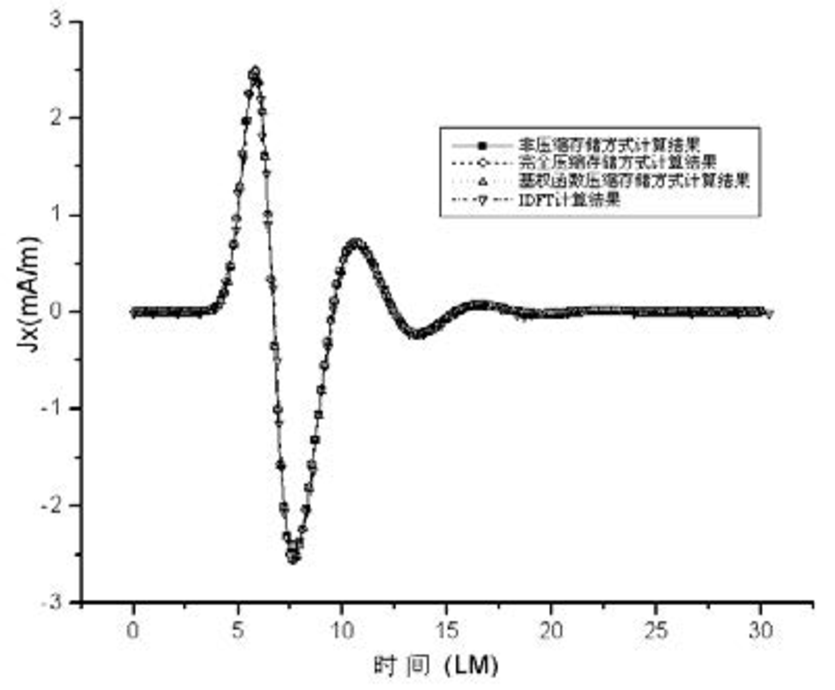
\includegraphics[width=6.77cm]{picd.pdf}
}
\subfloat[]{
    \label{pice}
    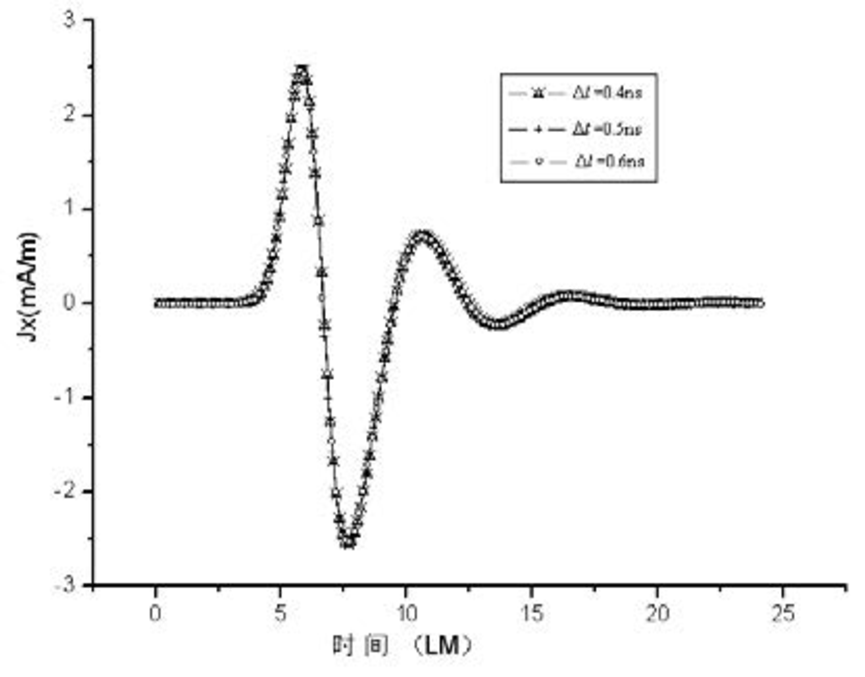
\includegraphics[width=7.04cm]{pice.pdf}
}
\caption{$2m\times 2m$的理想导体平板中心处感应电流$x$分量随时间的变化关系。(a)不同存储方式的计算结果与IDFT方法的结果比较;(b)不同时间步长的计算结果比较比较比较}
\label{fig2}
\end{figure}

由于时域混合场积分方程是时域电场积分方程与时域磁场积分方程的线性组合,因此时域混合场积分方程时间步进算法的阻抗矩阵特征与时域电场积分方程时间步进算法的阻抗矩阵特征相同。

\section{时域积分方程时间步进算法矩阵方程的求解}
\begin{theorem}
如果时域混合场积分方程是时域电场积分方程与时域磁场积分方程的线性组合。
\end{theorem}
\begin{proof}
由于时域混合场积分方程是时域电场积分方程与时域磁场积分方程的线性组合,因此时域混合场积分方程时间步进算法的阻抗矩阵特征与时域电场积分方程时间步进算法的阻抗矩阵特征相同。
\end{proof}
\begin{corollary}
时域积分方程方法的研究近几年发展迅速,在本文研究工作的基础上,仍有以下方向值得进一步研究。
\end{corollary}
\begin{lemma}
因此时域混合场积分方程时间步进算法的阻抗矩阵特征与时域电场积分方程时间步进算法的阻抗矩阵特征相同。
\end{lemma}

\section{本章小结}
本章首先研究了时域积分方程时间步进算法的阻抗元素精确计算技术,分别采用DUFFY变换法与卷积积分精度计算法计算时域阻抗元素,通过算例验证了计算方法的高精度。
